\subsubsection{Affine Space and Affine Curves}
The main object of interest in this subsection is the projective plane.
Before we introduce it, though, we begin with a prerequisite definition.

\begin{definition}
	Let $k$ be an algebraically closed field. Define affine $n$-space, or $\an$, to be the set of all $n$-tuples, or points,
	$$\an = \{ (a_1,a_2,\ldots,a_n) | a_i \in k\}.$$
\end{definition}

The consideration of algebraically closed fields differentiates affine space from $\R^n$, where from now on, unless otherwise mentioned, we take the field $k = \C$.
% note about how we don't need to use C necessarily?
We call affine 2-space, or $\an[2]$, the \emph{affine plane}.

In affine $n$-space, it is possible to define \emph{affine curves} in the following way.
\begin{definition}
	In $\an$, for a given polynomial $f$ in $n$ variables $x_1,\ldots,x_n$, an \emph{affine curve} is the set $V(f)$ of all points $(x_1,\ldots,x_n)$ such that $f(x_1,\ldots,x_n)=0$. More concisely,
	$$V(f) = \{(x_1,\ldots,x_n) | f(x_1,\ldots,x_n)=0$$
\end{definition}
\Cref{affinecurveexample} shows an example of an affine curve.

% unfinished diagram
\begin{figure}[htbp]
	\centering
	\begin{tikzpicture}[scale=0.5,domain=-5:5]
		% axes
		\draw[->] (-5,0) -- (5,0);
		\draw[->] (0,-5) -- (0,5);
		\node [right] at (5,0) {$x$};
		\node [right] at (0,5) {$y$};
		% graph
		\draw 
		plot (\x, {\x});
	\end{tikzpicture}
	\caption{The affine curve $x^3 - 2xy = 0$ in the visible part of $\an[2]$}
	\label{affinecurveexample}
\end{figure}

It is important to distinguish the two objects $V(f)$ and $f$, as $f$ is simply a polynomial, whereas $V(f)$ is the set of points that are a solution to a polynomial \emph{equation} $f(x_1,\ldots,x_n)=0$.
However, for convenience, we write the curve $V(f)$ as its defining polynomial equation $f(x,y)=0$, when it is clear to do so.
The distinction of objects remains, though, and this is purely notational.

More points on notation are that in the affine plane, instead of $x_1$ and $x_2$, we write $x$ and $y$, lowercase.
We also write polynomials as lowercase letters $f$, $g$ etc.
The reason for this will be explained shortly.
\subsubsection{Projective Space}
Now that affine space has been introduced, we are ready to introduce projective $n$-space $\pn$, and with that, the projective plane $\pn[2]$.

The projective plane is an idea that grew out of the renaissance study of perspective in art.
For example, when stood between two railway lines, they appear to meet at the horizon.
\Cref{projective-parallel} is a diagram of the situation.
While this is merely a trick of perspective in euclidean space, in the projective plane, parallel lines \emph{do} meet, at a so called `point at infinity'.
% euclidean/affine? What?
The idea is to add these points at infinity to the affine plane so that each line contains exactly one.
On top of this is the one exception, the `line at infinity', which is defined to be the unique line that is simply the collection of all points at infinity.
These ideas, while formative, are not rigorous, and we present the proper definition and constructions (there are two) of projective space below.

\begin{figure}[htbp]
	\centering
	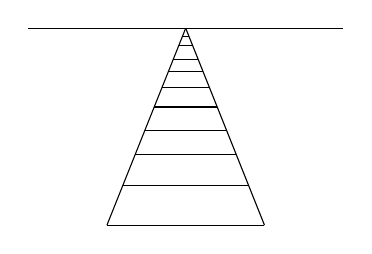
\begin{tikzpicture}[scale=0.5]
		% railway lines
		\draw (-2,0) -- (0,5);
		\draw (2,0) -- (0,5);
		% sleepers. To work out an appropriate x for given y, x=2(1-(y/5))
		\draw (-2,0) -- (2,0);
		\draw (-1.6,1) -- (1.6,1);
		\draw (-1.28,1.8) -- (1.28,1.8);
		\draw (-1.04,2.4) -- (1.04,2.4);
		\draw (-0.8,3) -- (0.8,3);
		\draw (-0.6,3.5) -- (0.6,3.5);
		\draw (-0.44,3.9) -- (0.44,3.9);
		\draw (-0.32,4.2) -- (0.32,4.2);
		\draw (-0.18,4.55) -- (0.18,4.55);
		\draw (-0.08,4.8) -- (0.08,4.8);
		% horizon
		\draw (-4,5) -- (4,5);
	\end{tikzpicture}
	\caption{Parallel lines `meeting' at infinity in euclidean space}
	\label{projective-parallel}
\end{figure}

% \begin{definition}
% 	The projective plane is an extension of the affine plane $\an[2]$ created by adding `points at infinity' such that every pair of lines intersects exactly once.
% 	Points in projective $n$-space are represented by $n+1$-tuples modulo an equivalence relation, such that not all coordinates are zero.
% \end{definition}

The two constructions of projective space give two different interpretations of it, both of which are useful to consider.
Projective $n$-space can be thought of as either affine $n$-space with points at infinity added (mentioned already) or as a quotient of affine $(n+1)$-space.

\subsubsection{Construction 1: Quotient of $\an[n+1]$}
Remove the origin (i.e. the point $(0,0,\ldots,0)$) from $\an[n+1]$ and define an equivalence relation $\sim$ on the remaining points as follows:
$$(a_0,a_1,\ldots,a_n) \sim (b_0,b_1,\ldots,b_n) \iff (a_0,a_1,\ldots,a_n) = \lambda(b_0,b_1,\ldots,b_n)$$
where $\lambda$ is a non-zero scalar in $\C$. Then we have 
$$\pn = (\an[n+1]\setminus\{(0,\ldots,0)\})/\sim,$$
the set of equivalence classes of $\sim$.

Therefore, we see that points in $\pn$ are equivalence classes of lines in $\an[n+1] \setminus \{0\}$.
For points in $\pn$, write $P = [p_0,p_1,\ldots,p_n]$, where the square brackets represent the \emph{homogeneous coordinates} of the point.
We see that $[p_0,p_1,\ldots,p_n] = \{(\lambda a_0, \lambda a_1,\ldots,\lambda a_n | \lambda \in \C\}$.

By the nature of this construction, it is clear that scaling homogeneous coordinates results in coordinates of the same point.
Therefore, for a given point, there is no unique representation in homogeneous coordinates, and we may scale coordinates for our convenience.

\subsubsection{Construction 2: Extension of $\an[n]$}
Now we present the second construction of $\pn$, which can be thought of as adding points at infinity to affine $n$-space.
This is done inductively on $n$ by defining maps $\alpha_n$ and $\beta_n$.
To begin with, let $\pn[0] = \an[1] \setminus \{0\}$ and let
\begin{alignat*}{2}
&\alpha_n : \an \rightarrow \pn,\quad &&\alpha_n(x_1,\ldots,x_n) = [x_1,\ldots,x_n,1]\\
 &\beta_n : \pn[n-1] \rightarrow \pn,\quad &&\beta_n[X_1,\ldots,X_n] = [X_1,\ldots,X_n,0]
\end{alignat*}
Then we can define
$$\pn = \alpha_n(\an) \cup \beta_n(\pn[n-1])$$
Effectively, we have that $\alpha_n$ is the embedding of affine space in $\pn$ and $\beta_n$ represents the points at infinity of $\pn$.
Notice that the image of $\beta_n$ will always give valid homogeneous coordinates, as we removed zero from $\pn[0]$, and therefore at least one of the first $n$ coordinates will be nonzero.
\subsubsection{Homogenisation of Polynomials}
Now that projective space has been introduced, it is natural to wonder what form curves in projective space take.
If we try to define projective curves in $\pn$ in the same way as affine curves, i.e. as solutions of a polynomial equation $f(x_1,\ldots,x_n)=0$ in $n$ variables, we find that it is not always possible, since we saw that the homogeneous coordinates of a point are not unique.
For example, if we tried to define a projective curve as $F(X,Y,Z)=X^2+Y+Z=0$, we see that $[2,-2,-2]$ is a solution of this equation, and so $[2,-2,-2] \in F$.
However, since we work with homogeneous coordinates, the point $[2,-2,-2]$ is also be written as $[-2,2,2]$, which clearly does not satisfy $F(X,Y,Z)=0$.
This is a problem, as we do not want the representation of a point to affect whether it lies on a curve or not.

To that extent, when working with the projective plane, it is convenient to define a homogeneous polynomial as a polynomial which satisfies
$$F(tX_1,tX_2,\ldots,tX_n)=t^k F(X_1,X_2,\ldots,X_n)$$
for some $t \in \C$ and $k \in \N$. We see that these kinds of polynomials are able to define curves in the projective plane, as for a homogeneous polynomial $F$,
$$F(X_1,X_2,\ldots,X_n)=0 \Leftrightarrow F(tX_1,tX_2,\ldots,tX_n) = t^k F(X_1,X_2,\ldots,X_n) = 0$$

It is easy enough to see that a polynomial is homogeneous if and only if the degree of each monomial $= d$, for some $d \in \N$.
So the polynomial $\frac{1}{2}x^4 + x^2y^2 + 14xy^3$ is homogeneous with degree 4, whereas the polynomial $17x^5 + 12x^2y + 2$ is not, as the monomials have degrees 5, 3 and 0, from left-to-right.

It is possible to homogenise a given polynomial $f(x_1,\ldots,x_n)$ by letting
$$F = F(X_1,X_2,\ldots,X_{n+1}) = (X_{n+1})^d f(\frac{X_1}{X_{n+1}},\ldots,\frac{X_n}{X_{n+1}}),$$
where $d$ is the maximum degree of all monomials of $F$.
In practice, this resembles `topping up' the monomials with an extra variable as necessary.
So the inhomogeneous polynomial $17x^5 + 12x^2y + 2$ discussed earlier can be homogenised as $17X^5 + 12X^2YZ^2 + 2Z^5$.
The reverse transition can be made also, simply by letting $f = f(x_1,\ldots,x_n) = F(x_1,\ldots,x_n,1)$, which looks like simply taking out the extra variable.

There are a few things to notice here.
First, when writing out projective polynomials, we use uppercase letters to distinguish them from affine variables and make the context clear.
We also use $X$, $Y$ and $Z$ (and also $x$ and $y$) as the three variables when dealing with the projective plane (uppercase) and the affine part thereof (lowercase).

To summarise, it is possible to move to and from the projective plane with regards to both points and polynomials.
A point $(x,y)$ can be mapped to $[x,y,1]$, and from $[X,Y,Z]$ to $(X/Z,Y/Z)$.
A polynomial $f(x,y)$ can be mapped to $F(X,Y,Z) = Z^d f(x/Z,y/Z)$, and back by mapping $F(X,Y,Z)$ to $f(x,y) = F(x,y,1)$.

\begin{figure}[htbp]
	\centering
	\begin{tikzpicture}[scale=0.5,domain=-5:5]
		% axes
		\draw[->] (-5,0) -- (5,0);
		\draw[->] (0,-5) -- (0,5);
		\node [right] at (5,0) {$x$};
		\node [right] at (0,5) {$y$};
		% lines
		\draw 
		plot (\x, {0.5*\x+1});
		\draw 
		plot (\x, {0.5*\x+4});
		% annotation
		\draw[dashed,->]
		plot (\x, {0.5*\x+2.5});
		\node [right] at (5,5) {[3,-2,0]};
	\end{tikzpicture}
	\caption{The intersection of $2x - 3y + 1 = 0$ and $2x - 3y + 4 = 0$}
	\label{euclidean-intersection}
\end{figure}
The lines given by $2x - 3y + 1 = 0$ and $2x - 3y + 4 = 0$, which are parallel in $\R^2$, intersect in the projective plane at the point [3,-2,0].
This is because, when homogenised with respect to $z$, the curves are given by $2X - 3Y + Z = 0$ and $2X - 3Y + 4Z = 0$, which are clearly satisfied by $[X,Y,Z] = [3,-2,0]$.
\subsubsection{Projective Curves}
Now that the basics of projective geometry have been established, we introduce a few more ideas necessary for understanding the main subject matter.
From now on, we also limit ourselves to the projective plane $\pn[2]$.

\begin{definition}
	A projective curve is the set of points defined by a \emph{homogeneous} polynomial equation $F(X_1,X_2,\ldots,X_n) = 0$.
	When discussing the projective plane $\pn[2]$, we write $F(X,Y,Z) = 0$.
\end{definition}
The degree of a curve is the degree of the polynomial in the defining equation.
For example, the polynomial equations $X^3-YZ^2=0$, $13X^2Z + Y^3 + 4XYZ = 0$ and $Z^2 + \frac{1}{2}Y^2 = 0$ all define projective curves in $\pn[2]$.
The first two have degree 3, the third, degree 2.

\begin{definition}
	A singular point on a curve $F$ is a point where all partial derivatives $F_X$, $F_Y$ and $F_Z$ vanish. A point that is not a singular point is called a regular point.
\end{definition}
Two good examples of projective curves with singular points are provided by the \emph{cusp} $C : Y^2Z - X^3$ and the \emph{node} $N : Y^2Z - X^3 - X^2Z$, which are illustrated in \Cref{cuspandnode}.
\begin{figure}[htbp]
	\centering
	\begin{tikzpicture}[scale=0.5,domain=-5:5]
		% axes
		\draw[->] (-5,0) -- (5,0);
		\draw[->] (0,-5) -- (0,5);
		\node [right] at (5,0) {$x$};
		\node [right] at (0,5) {$y$};
		% graph
		\draw 
		plot (\x, {\x});
	\end{tikzpicture}
	\caption{The cusp and node in the visible part of $\an[2]$}
	\label{cuspandnode}
\end{figure}
We can see that the point $[0,0,1]$ (the origin in the affine plane) is a singular point on both curves, since
\begin{alignat*}{2}
	&C_X = -3X^2,\qquad &&N_X = - 3X^2 - 2XZ\\
	&C_Y = 2YZ,\qquad &&N_Y = 2YZ\\
	&C_Z = Y^2,\qquad &&N_Z = Y^2 -X^2,
\end{alignat*}
and all partial derivatives vanish at zero.

Singular points are important to consider as they are the points where there is no sensible notion of the tangent to a curve.
The importance of this will become apparent later on.
An alternative characterisation of a singular point is that the intersection multiplicity of a line and the curve at that point is always greater than one.

Supposing that a point on a curve is regular, and therefore has a tangent.
It is possible to find the equation of the line by examining the partial derivatives of the curve.
For example, let $F: X^3 - 3XZ^2 - Y^2Z = 0$ and consider the point $[0,1,0]$ on $F$.
We have $F_X(X,Y,Z) = 3X^2 -3Z^2$, $F_Y(X,Y,Z) = -2YZ$ and $F_Z(X,Y,Z) = -6XZ - Y^2$.
The equation of the tangent line $L$ is given by
$$L : F_X(P)X + F_Y(P)Y + F_Z(P)Z = 0$$
In this case, we have $L : -X - Z = 0$, or $L: X + Z = 0$.
As alluded to before, being able to find tangent lines plays an important part in our upcoming material.

\begin{definition}
	A curve that contains one or more singular points is a singular curve. Otherwise, the curve is regular.
\end{definition}

\begin{definition}
	A \emph{flex} is a point $P$ on a curve $F$ where the tangent to $F$ at $P$ intersects $F$ with multiplicity at least 3.
\end{definition}

Flexes are important points
